% Fonte editável de fig/hv_ilustracao_pt.pdf (Figura do cálculo do HV,
% Cap. 2, Seção 2.4.2). Esquemática: os pontos são ilustrativos e não vêm de
% nenhuma execução, e são as mesmas duas aproximações de
% fig/src/igd_ilustracao_pt.tex. Plano normalizado, minimização dos dois
% objetivos, ponto de referência r = (1, 1), como na Seção sec:metricas.
% Cada solução a domina o retângulo [a, r]; a região cinza é a união desses
% retângulos (Equação eq:hv), traçada como escada pelas soluções ordenadas
% em f1. O contorno espesso é o retângulo de uma única solução. Com estes
% pontos, HV(a) = 0,502 e HV(b) = 0,267. Os valores não aparecem na figura;
% servem para conferir o rótulo qualitativo de cada painel.
%
% Regenerar, a partir de thesis/masters/ (a primeira compilação baixa o TikZ;
% o build da dissertação só inclui o PDF e continua offline):
%   tectonic -o fig fig/src/hv_ilustracao_pt.tex
\documentclass[border=2pt]{standalone}
\usepackage{fontspec}
\setmainfont{texgyreheros}[
  Extension = .otf,
  UprightFont = *-regular,
  BoldFont = *-bold,
]
\usepackage{tikz}
\usetikzlibrary{arrows.meta}

% (a) aproximação distribuída:
\def\distribuida{0.04/0.8700, 0.24/0.5801, 0.48/0.3772, 0.72/0.2215, 0.94/0.1005}
% (b) aproximação concentrada:
\def\concentrada{0.7/0.1783, 0.76/0.1432, 0.83/0.1040, 0.9/0.0663, 0.97/0.0301}

\tikzset{
  solucao/.style={circle, draw=black, fill=black, inner sep=0pt, minimum size=5.2pt},
  ref/.style={rectangle, draw=black, fill=white, line width=0.8pt, inner sep=0pt, minimum size=6pt},
  dominada/.style={fill=black!15, draw=black!55, line width=0.5pt},
  individual/.style={draw=black, line width=1.1pt},
  fronteira/.style={black!30, line width=0.8pt},
  titulo/.style={anchor=south west, font=\bfseries, inner sep=0pt},
  rotulo/.style={anchor=south west, inner sep=0pt},
}

\newcommand{\eixos}{%
  \draw[-{Latex[length=2mm]}, line width=0.6pt] (0,0) -- (1.12,0) node[below, inner sep=2pt] {$f_1$};
  \draw[-{Latex[length=2mm]}, line width=0.6pt] (0,0) -- (0,1.12) node[left, inner sep=2pt] {$f_2$};
  \draw[line width=0.6pt] (1,0) -- ++(0,-0.02) node[below, inner sep=1.5pt] {$1$};
  \draw[line width=0.6pt] (0,1) -- ++(-0.02,0) node[left, inner sep=1.5pt] {$1$};
  \node[below left, inner sep=1.5pt] at (0,0) {$0$};
}

\newcommand{\pontoref}{%
  \node[ref] at (1,1) {};
  \node[anchor=south west, inner sep=3pt] at (1,1) {$\mathbf{r}$};
}

\begin{document}
\fontsize{9}{11}\selectfont
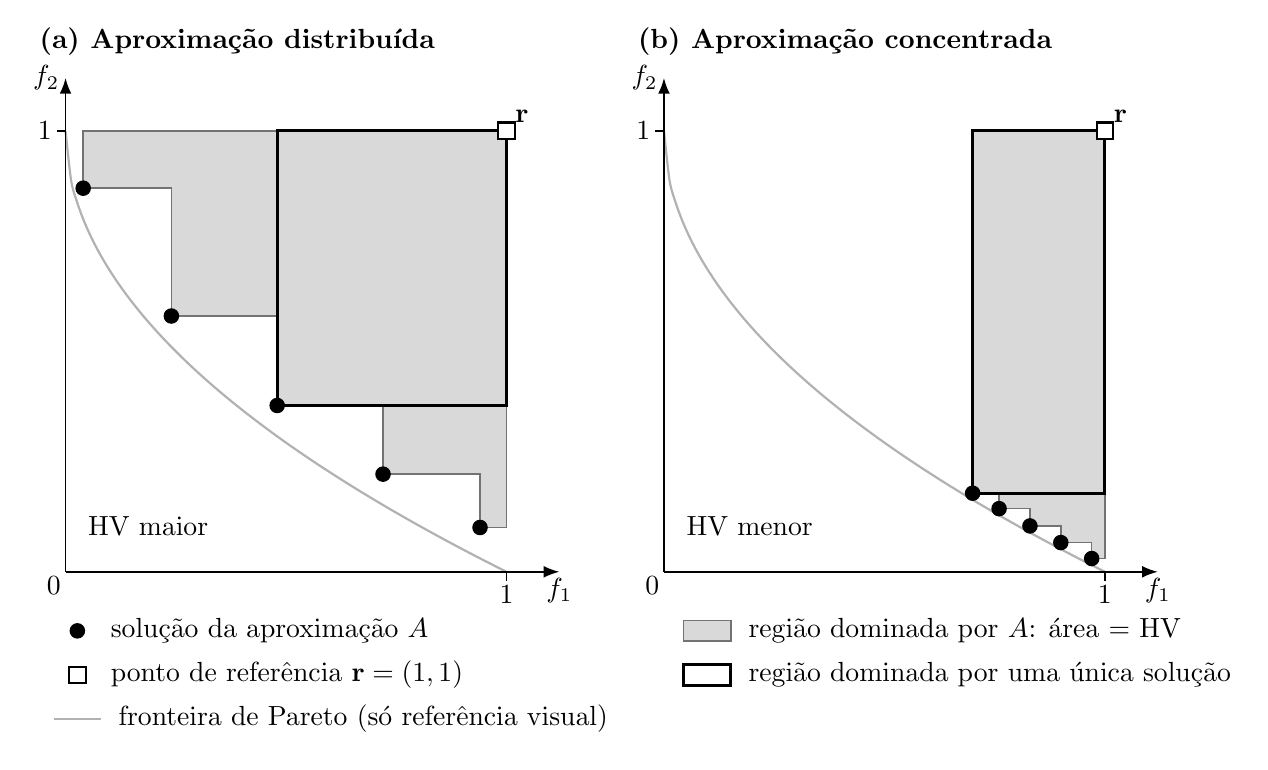
\begin{tikzpicture}[x=5.6cm, y=5.6cm]

  % ---------------- (a) aproximação distribuída ----------------
  \begin{scope}
    \draw[dominada] (0.04,1) -- (0.04,0.8700) -- (0.24,0.8700) -- (0.24,0.5801)
      -- (0.48,0.5801) -- (0.48,0.3772) -- (0.72,0.3772) -- (0.72,0.2215)
      -- (0.94,0.2215) -- (0.94,0.1005) -- (1,0.1005) -- (1,1) -- cycle;
    \draw[fronteira] plot[domain=0:1, samples=80, smooth] (\x, {1 - sqrt(\x)});
    \eixos
    \draw[individual] (0.48,0.3772) rectangle (1,1);
    \foreach \x/\y in \distribuida { \node[solucao] at (\x,\y) {}; }
    \pontoref
    \node[titulo] at (-0.06,1.17) {(a) Aproximação distribuída};
    \node[rotulo] at (0.05,0.08) {HV maior};
  \end{scope}

  % ---------------- (b) aproximação concentrada ----------------
  \begin{scope}[xshift=7.6cm]
    \draw[dominada] (0.7,1) -- (0.7,0.1783) -- (0.76,0.1783) -- (0.76,0.1432)
      -- (0.83,0.1432) -- (0.83,0.1040) -- (0.9,0.1040) -- (0.9,0.0663)
      -- (0.97,0.0663) -- (0.97,0.0301) -- (1,0.0301) -- (1,1) -- cycle;
    \draw[fronteira] plot[domain=0:1, samples=80, smooth] (\x, {1 - sqrt(\x)});
    \eixos
    \draw[individual] (0.7,0.1783) rectangle (1,1);
    \foreach \x/\y in \concentrada { \node[solucao] at (\x,\y) {}; }
    \pontoref
    \node[titulo] at (-0.06,1.17) {(b) Aproximação concentrada};
    \node[rotulo] at (0.05,0.08) {HV menor};
  \end{scope}

  % ---------------- legenda ----------------
  \begin{scope}[x=1cm, y=1cm, shift={(0,-0.75)}]
    \def\lin{0.56}
    \node[solucao] at (0.15,0) {};   \node[anchor=west] at (0.45,0) {solução da aproximação $A$};
    \node[ref] at (0.15,-\lin) {};   \node[anchor=west] at (0.45,-\lin) {ponto de referência $\mathbf{r} = (1, 1)$};
    \draw[fronteira] (-0.15,-2*\lin) -- (0.45,-2*\lin); \node[anchor=west] at (0.55,-2*\lin) {fronteira de Pareto (só referência visual)};
    \fill[black!15, draw=black!55, line width=0.5pt] (7.85,-0.13) rectangle (8.45,0.13);
    \node[anchor=west] at (8.55,0) {região dominada por $A$: área = HV};
    \draw[individual] (7.85,-\lin-0.13) rectangle (8.45,-\lin+0.13);
    \node[anchor=west] at (8.55,-\lin) {região dominada por uma única solução};
  \end{scope}
\end{tikzpicture}
\end{document}
